\documentclass[leqno]{article}

%% Created with wxMaxima 19.05.7

\setlength{\parskip}{\medskipamount}
\setlength{\parindent}{0pt}
\usepackage[utf8]{luainputenc}
\DeclareUnicodeCharacter{00B5}{\ensuremath{\mu}}
\usepackage{graphicx}
\usepackage{color}
\usepackage{amsmath}
\usepackage{ifthen}
\newsavebox{\picturebox}
\newlength{\pictureboxwidth}
\newlength{\pictureboxheight}
\newcommand{\includeimage}[1]{
    \savebox{\picturebox}{\includegraphics{#1}}
    \settoheight{\pictureboxheight}{\usebox{\picturebox}}
    \settowidth{\pictureboxwidth}{\usebox{\picturebox}}
    \ifthenelse{\lengthtest{\pictureboxwidth > .95\linewidth}}
    {
        \includegraphics[width=.95\linewidth,height=.80\textheight,keepaspectratio]{#1}
    }
    {
        \ifthenelse{\lengthtest{\pictureboxheight>.80\textheight}}
        {
            \includegraphics[width=.95\linewidth,height=.80\textheight,keepaspectratio]{#1}
            
        }
        {
            \includegraphics{#1}
        }
    }
}
\newlength{\thislabelwidth}
\DeclareMathOperator{\abs}{abs}
\usepackage{animate} % This package is required because the wxMaxima configuration option
                      % "Export animations to TeX" was enabled when this file was generated.

\definecolor{labelcolor}{RGB}{100,0,0}

\begin{document}

\pagebreak{}
{\Huge {\sc Simulation des Lorenz-Systems

}}
\setcounter{section}{0}
\setcounter{subsection}{0}
\setcounter{figure}{0}

Das Lorenz-System ist ein System dreier nichtlinearer Differentialgleichungenerster Ordnung mit folgenden Zustandsgleichungen:




\noindent
%%%%%%%%%%%%%%%
%%% INPUT:
\begin{minipage}[t]{4em}\color{red}\bf
(\% i3)
\end{minipage}
\begin{minipage}[t]{\textwidth}\color{blue}
l1: 'diff(x, t) = 10*(y - x);

l2: 'diff(y, t) = 28*x - y - x*z;

l3: 'diff(z, t) = x*y - 8/(3*z);


\end{minipage}
%%% OUTPUT:
\[\displaystyle \tag{l1}
\frac{d}{d t} x=10 \left( y-x\right) \mbox{}\]

\[\tag{l2}
\frac{d}{d t} y=-x z-y+28 x\mbox{}\]

\[\tag{l3}
\frac{d}{d t} z=x y-\frac{8}{3 z}\mbox{}
\]
%%%%%%%%%%%%%%%
Dieses Gleichungssystem stellt ein stark vereinfachtes Modell für dasWettergeschehen dar, das von Edward N. Lorenz in den 1960er Jahren formuliertwurde. Das Besondere an diesem System ist, daß es chaotisch ist und eineoszillierende, aber nicht periodische Bewegung vollführt.


System dreier nichtlinearer Differentialgleichungen mit den Variablen x, y,z:




\noindent
%%%%%%%%%%%%%%%
%%% INPUT:
\begin{minipage}[t]{4em}\color{red}\bf
(\% i6)
\end{minipage}
\begin{minipage}[t]{\textwidth}\color{blue}
g1: 10*(y - x);

g2: 28*x - y - x*z;

g3: x*y - 8/3*z;


\end{minipage}
%%% OUTPUT:
\[\displaystyle \tag{g1}
10 \left( y-x\right) \mbox{}\]

\[\tag{g2}
-x z-y+28 x\mbox{}\]

\[\tag{g3}
x y-\frac{8 z}{3}\mbox{}
\]
%%%%%%%%%%%%%%%
Numerische Lösung der Differentialgleichung mit dem Runge-Kutta-Verfahren:




\noindent
%%%%%%%%%%%%%%%
%%% INPUT:
\begin{minipage}[t]{4em}\color{red}\bf
(\% i8)
\end{minipage}
\begin{minipage}[t]{\textwidth}\color{blue}
res1: rk([g1, g2, g3], [x, y, z], [7, 10, 18], [t, 0, 25, 0.01])\$


\end{minipage}

\noindent%

Das Ergebnis, eine geschachtelte Liste, wird in vier einzelne Listen zerlegt:




\noindent
%%%%%%%%%%%%%%%
%%% INPUT:
\begin{minipage}[t]{4em}\color{red}\bf
(\% i12)
\end{minipage}
\begin{minipage}[t]{\textwidth}\color{blue}
lit: map(first, res1)\$

lix: map(second, res1)\$

liy: map(third, res1)\$

liz: map(fourth, res1)\$


\end{minipage}

\noindent%

Setzen einiger Graphikoptionen als Default-Werte:




\noindent
%%%%%%%%%%%%%%%
%%% INPUT:
\begin{minipage}[t]{4em}\color{red}\bf
(\% i13)
\end{minipage}
\begin{minipage}[t]{\textwidth}\color{blue}
set\_draw\_defaults(point\_type = 0, point\_size = 0,

points\_joined = true, color = red, grid = true);


\end{minipage}
%%% OUTPUT:
\[\displaystyle \tag{\% o13} 
[\mathit{point\_ type}=0,\mathit{point\_ size}=0,\mathit{points\_ joined}=\mbox{true},\mathit{color}=\mathit{red},\mathit{grid}=\mbox{}\\\mbox{true}]\mbox{}
\]
%%%%%%%%%%%%%%%
Darstellung der Variablen x (rot), y (blau) und z (grün) in Abhängigkeit von derZeit t:




\noindent
%%%%%%%%%%%%%%%
%%% INPUT:
\begin{minipage}[t]{4em}\color{red}\bf
(\% i14)
\end{minipage}
\begin{minipage}[t]{\textwidth}\color{blue}
wxdraw2d(points(lit, lix), color = blue, points(lit, liy), color = green,

points(lit, liz))\$


\end{minipage}
%%% OUTPUT:
\[\displaystyle \tag{\% t14} 
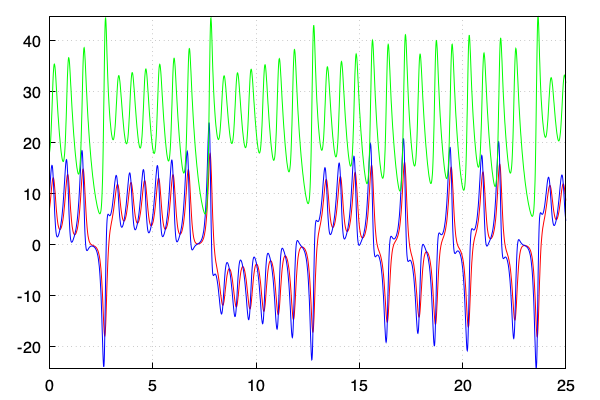
\includegraphics[width=.95\linewidth,height=.80\textheight,keepaspectratio]{lorenz_img/lorenz_1}\mbox{}
\]
%%%%%%%%%%%%%%%
Parameterdarstellung der Lösung in der xz-Ebene:




\noindent
%%%%%%%%%%%%%%%
%%% INPUT:
\begin{minipage}[t]{4em}\color{red}\bf
(\% i15)
\end{minipage}
\begin{minipage}[t]{\textwidth}\color{blue}
wxdraw2d(points(lix, liz))\$


\end{minipage}
%%% OUTPUT:
\[\displaystyle \tag{\% t15} 
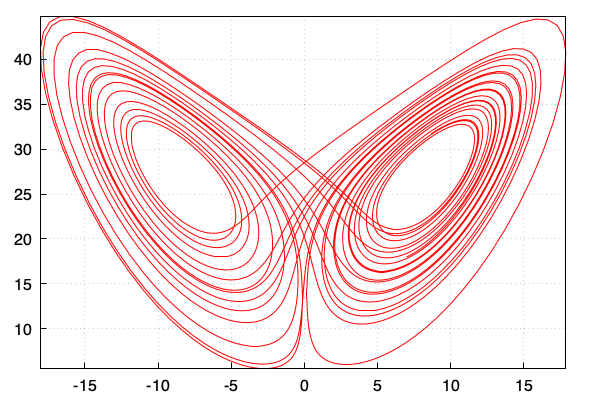
\includegraphics[width=.95\linewidth,height=.80\textheight,keepaspectratio]{lorenz_img/lorenz_2}\mbox{}
\]
%%%%%%%%%%%%%%%


\noindent
%%%%%%%%%%%%%%%
%%% INPUT:
\begin{minipage}[t]{4em}\color{red}\bf
 \ensuremath{\longrightarrow}  
\end{minipage}
\begin{minipage}[t]{\textwidth}\color{blue}

\end{minipage}

\noindent%

\end{document}
